\section{Use case} \label{sec:usecase} 
På baggrund af systembeskrivelsen samt opstillede krav er der udarbejdet et use case diagram, der beskriver app'ens funktioner. Af use case diagrammet på \autoref{fig:usecase} ses systemet, app til KOL-patienter, samt de forskellige use cases og aktører, der kan interagere med systemet. KOL-patienten er den primære aktør, som kan tilgå alle use cases. Målinger, database, sundhedspersonale og andre KOL-patienter er sekundære aktører og kan kun tilgå enkelte use cases. 

\begin{figure} [H]
\centering
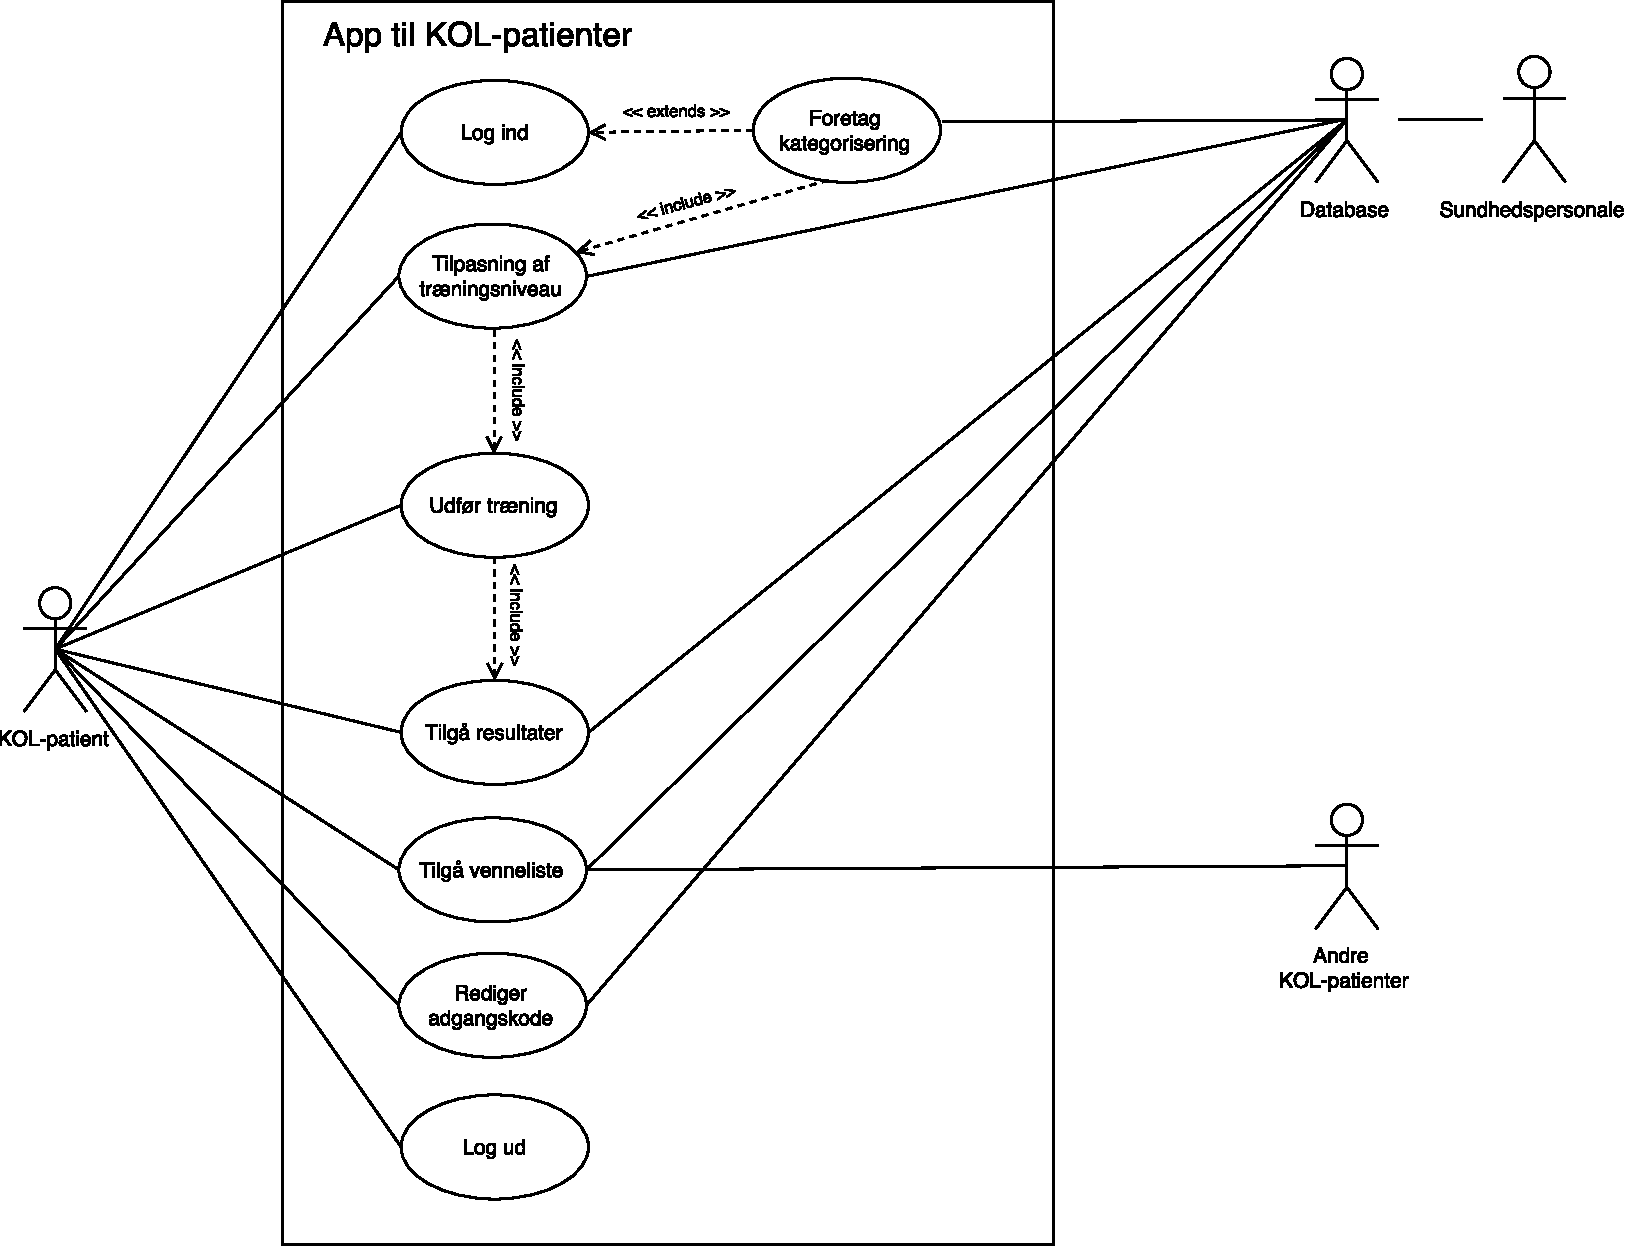
\includegraphics[width=0.9\textwidth]{figures/aktivitetsdiagram/Usecase}
\caption{Use case for app til KOL-patienter}
\label{fig:usecase}
\end{figure}

\noindent
Efter KOL-patienter er logget ind i app'en har de adgang til en hovedmenu, hvorfra brugere kan vælge at redigere brugeroplysninger, udføre træning, se resultater og venneliste. 

I \textit{Redigering af brugeroplysninger} kan brugere redigere deres adgangskode og kategorisering. Det skal være muligt for brugeren at ændre disse, da de ved registrering får en adgangskode udleveret. Dertil skal det være muligt at gøre deres adgangskode personligt. Derudover kan deres tilstand grundet KOL ændres, hvorfor kategoriseringen skal kunne redigeres. Hvis der foretages ændringer gemmes disse efterfølgende i databasen. 

\textit{Valg af træningsniveau} tilpasses individuelt ud fra \textit{Patientstatus}, der vurderes ud fra \textit{Kategorisering}, \textit{Daglig helbredstilstand} samt \textit{Evaluering af træning}.
Under \textit{Træning} kan eksterne enheder tilkobles systemet, således målinger kan opsamles. Ved en udført træning startes en nedtælling, som efter 24 timer sender en \textit{Notifikation} med henblik på at motivere brugeren til træning. Hvis brugeren benytter app'en førend de 24 timer er gået, nulstilles timeren.
Efter udført træning samt evaluering gemmes patientens status, træningsresultater samt målinger i \textit{Resultater} og databasen. 
Brugere kan tilgå samtlige resultater, som visualiseres i en kalender, ved grafisk udvikling samt belønninger. Sundhedspersonalet kan kun tilgå udviklingen af brugerens træning, mens brugeren via \textit{Venneliste} kan vælge at tilgå andres belønninger. Dette medvirker til, at brugere kan motivere hinanden til at udføre træning. Efter hver handling returneres brugeren til hovedmenuen.